\documentclass[11pt]{article}

\newcommand{\yourname}{Kevin Zhang}

\def\comments{0}

%format and packages

%\usepackage{algorithm, algorithmic}
\usepackage{graphicx}
\usepackage{forest}
\usepackage{tikz}
\usepackage{algpseudocode}
\usepackage{amsmath, amssymb, amsthm}
\usepackage{tcolorbox}
\usepackage{enumerate}
\usepackage{enumitem}
\usepackage{framed}
\usepackage{verbatim}
\usepackage[margin=1.0in]{geometry}
\usepackage{microtype}
\usepackage{kpfonts}
\usepackage{palatino}
	\DeclareMathAlphabet{\mathtt}{OT1}{cmtt}{m}{n}
	\SetMathAlphabet{\mathtt}{bold}{OT1}{cmtt}{bx}{n}
	\DeclareMathAlphabet{\mathsf}{OT1}{cmss}{m}{n}
	\SetMathAlphabet{\mathsf}{bold}{OT1}{cmss}{bx}{n}
	\renewcommand*\ttdefault{cmtt}
	\renewcommand*\sfdefault{cmss}
	\renewcommand{\baselinestretch}{1.06}

\usepackage[boxruled,vlined,nofillcomment]{algorithm2e}
	\SetKwProg{Fn}{Function}{\string:}{}
	\SetKwFor{While}{While}{}{}
	\SetKwFor{For}{For}{}{}
	\SetKwIF{If}{ElseIf}{Else}{If}{:}{ElseIf}{Else}{:}
	\SetKw{Return}{Return}
	

%enclosure macros
\newcommand{\paren}[1]{\ensuremath{\left( {#1} \right)}}
\newcommand{\bracket}[1]{\ensuremath{\left\{ {#1} \right\}}}
\renewcommand{\sb}[1]{\ensuremath{\left[ {#1} \right\]}}
\newcommand{\ab}[1]{\ensuremath{\left\langle {#1} \right\rangle}}

%probability macros
\newcommand{\ex}[2]{{\ifx&#1& \mathbb{E} \else \underset{#1}{\mathbb{E}} \fi \left[#2\right]}}
\newcommand{\pr}[2]{{\ifx&#1& \mathbb{P} \else \underset{#1}{\mathbb{P}} \fi \left[#2\right]}}
\newcommand{\var}[2]{{\ifx&#1& \mathrm{Var} \else \underset{#1}{\mathrm{Var}} \fi \left[#2\right]}}

%useful CS macros
\newcommand{\poly}{\mathrm{poly}}
\newcommand{\polylog}{\mathrm{polylog}}
\newcommand{\zo}{\{0,1\}}
\newcommand{\pmo}{\{\pm1\}}
\newcommand{\getsr}{\gets_{\mbox{\tiny R}}}
\newcommand{\card}[1]{\left| #1 \right|}
\newcommand{\set}[1]{\left\{#1\right\}}
\newcommand{\negl}{\mathrm{negl}}
\newcommand{\eps}{\varepsilon}
\DeclareMathOperator*{\argmin}{arg\,min}
\DeclareMathOperator*{\argmax}{arg\,max}
\newcommand{\eqand}{\qquad \textrm{and} \qquad}
\newcommand{\ind}[1]{\mathbb{I}\{#1\}}
\newcommand{\sslash}{\ensuremath{\mathbin{/\mkern-3mu/}}}
\newcommand{\pipe}{\hspace{3pt}|\hspace{3pt}}

%mathbb
\newcommand{\N}{\mathbb{N}}
\newcommand{\R}{\mathbb{R}}
\newcommand{\Z}{\mathbb{Z}}
%mathcal
\newcommand{\cA}{\mathcal{A}}
\newcommand{\cB}{\mathcal{B}}
\newcommand{\cC}{\mathcal{C}}
\newcommand{\cD}{\mathcal{D}}
\newcommand{\cE}{\mathcal{E}}
\newcommand{\cF}{\mathcal{F}}
\newcommand{\cL}{\mathcal{L}}
\newcommand{\cM}{\mathcal{M}}
\newcommand{\cO}{\mathcal{O}}
\newcommand{\cP}{\mathcal{P}}
\newcommand{\cQ}{\mathcal{Q}}
\newcommand{\cR}{\mathcal{R}}
\newcommand{\cS}{\mathcal{S}}
\newcommand{\cU}{\mathcal{U}}
\newcommand{\cV}{\mathcal{V}}
\newcommand{\cW}{\mathcal{W}}
\newcommand{\cX}{\mathcal{X}}
\newcommand{\cY}{\mathcal{Y}}
\newcommand{\cZ}{\mathcal{Z}}

%theorem macros
\newtheorem{thm}{Theorem}
\newtheorem{lem}[thm]{Lemma}
\newtheorem{fact}[thm]{Fact}
\newtheorem{clm}[thm]{Claim}
\newtheorem{rem}[thm]{Remark}
\newtheorem{coro}[thm]{Corollary}
\newtheorem{prop}[thm]{Proposition}
\newtheorem{conj}[thm]{Conjecture}

\theoremstyle{definition}
\newtheorem{defn}[thm]{Definition}
\newtheoremstyle{case}{}{}{}{}{}{:}{ }{}
\theoremstyle{case}
\newtheorem{case}{Case}

\theoremstyle{theorem}
\newtheorem{prob}{Problem}
\newtheorem{sol}{Solution}

\tikzset{every picture/.style={line width=0.75pt}} %set default line width to 0.75pt        

\begin{document}
{\large
\noindent \yourname \\
\noindent Assignment 1}


\vspace{15pt}

% Problem 1
\begin{prob}\end{prob}

\begin{enumerate}[label=(\alph*)]

% Part A
\item $N$ is the number of unordered pairs of distinct keys in $[U]$. This means $N = \binom{U}{2}$.
Next, we want to find the expected number of unordered pairs of distinct keys $x$ and $y$ such that $h(x) = h(y)$ when we 
pick a random hash function $h$ from $\mathcal{H}$ (Given that $\mathcal{H}$ is $c$-universal).

From the definition of $c$-universal, we know that $\underset{h \in \mathcal{H}}{Pr}[ h(x) = h(y) ] \leq \frac{c}{m}$.

Let $I_n$ be an indicator random variable that is 1 when $h(x) = h(y)$ and 0 otherwise for any given unordered pair of
distinct keys $x$ and $y$.

From this, we can determine $\mathbb{E}[I_n] \leq \frac{c}{m}$.

Let $I$ be the number of unordered pairs of distinct keys $x$ and $y$ where $h(x) = h(y)$. 

We can now express $\mathbb{E}[I]$:

\begin{align*}
            I &= \sum_{x \neq y}I_n \\
\mathbb{E}[I] &= \sum_{x \neq y}\mathbb{E}[I_n] \\
              &\leq N \cdot \frac{c}{m} \\
              &\leq \binom{U}{2} \cdot \frac{c}{m} \\
              &\leq \frac{U \cdot (U - 1) \cdot c}{2 \cdot m}
\end{align*}

% Part B
\item Let's consider one hash function $h \in \mathcal{H}$. Consider that $h$ maps $s_1$ number of 
distinct keys to value 1, and $s_2$ number of distinct keys to value 2, and so on, all the way to $s_m$. 
This means that for any value of $s_i$, there are exactly $\binom{s_i}{2}$ possible pairings of keys 
such that $h(x) = h(y)$. 

This let's us express $I$ differently:

\begin{align*}
  I &= \sum_{i = 1}^{m}\binom{s_i}{2} \\
    &= \sum_{i = 1}^{m}\frac{(s_i) \cdot (s_i - 1)}{2}
\end{align*}

% Part C
\item Now let's figure out $s_i$. For any given $s_i$, we know that $\mathbb{E}[s_i] \geq \frac{U}{m}$. This is because
we are trying to fit $U$ keys into $m$ spaces. We can now use the equation in part b to determine the following:

\begin{align*}
            I &= \sum_{i = 1}^{m}\frac{s_i \cdot (s_i - 1)}{2} \\
\mathbb{E}[I] &= \sum_{i = 1}^{m}\frac{\mathbb{E}[s_i] \cdot (\mathbb{E}[s_i] - 1)}{2} \\
              &\geq m \cdot \frac{\frac{U}{m} \cdot (\frac{U}{m} - 1)}{2} \\
              &\geq \frac{U \cdot (\frac{U}{m} - 1)}{2} 
\end{align*}

% Part D
\item By combining the inequalities of part A and part C, we can define a bound for the expected number of
unordered pairs of distinct keys $x$ and $y$ such that $h(x) = h(y)$ when we pick a random hash function $h \in \mathcal{H}$.

\[
  \frac{U \cdot (\frac{U}{m} - 1)}{2} \leq \mathbb{E}[I] \leq \frac{U \cdot (U - 1) \cdot c}{2 \cdot m}
\]

\end{enumerate}

% Problem 2
\begin{prob}\end{prob}

\begin{enumerate}[label=(\alph*)]

% Part A
\item We want to show that $f(x) = e^{tx}$ is convex for $t > 0$. By definition, a convex function
is also described such that all points along any line between two points on the function has a value greater than
or equal to the function value underneath the points. $f(x) = e^{tx}$ is convex over all t by
observation:

\begin{figure}[h!]
  \centering
  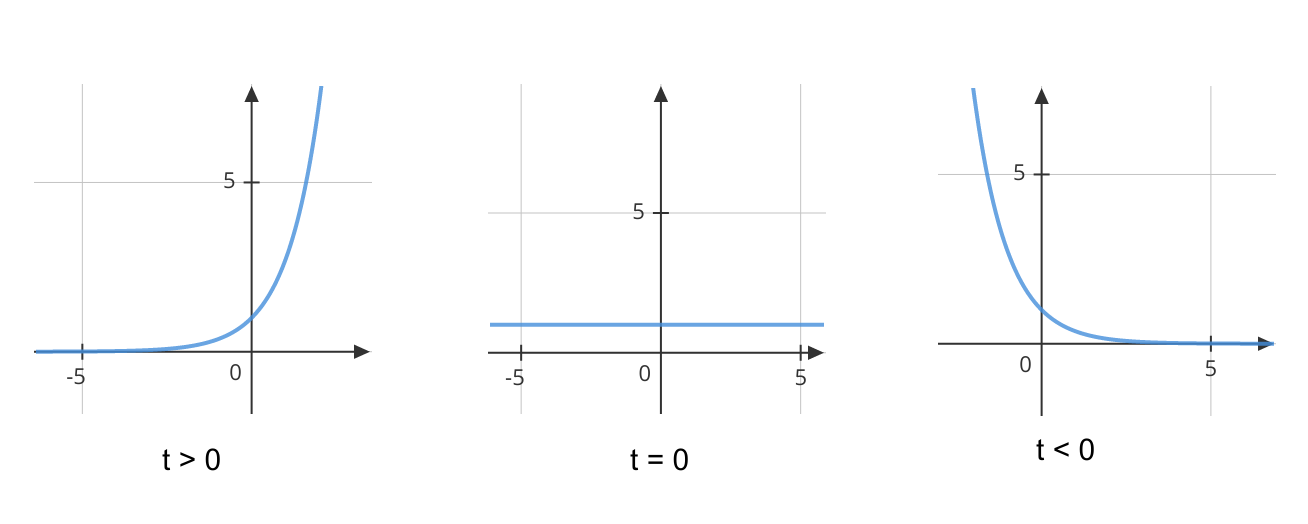
\includegraphics[totalheight=6cm]{images/convex.png}
\end{figure}

% Part B
\item Let $Z$ be a random variable with probability density function $g$ in the interval [0,1]. $p = \mathbb{E}[Z]$. 
Let's also define a Bernoulli random variable such that $Pr[X = 1] = p$. We want to show that for any convex
function $f$, the following is true.

\[
  \mathbb{E}[f(Z)] \leq \mathbb{E}[f(X)]
\] 

Let's start with the left hand side (LHS). We know that $\mathbb{E}[f(Z)] = \int_0^1 f(t) g(t) dt$ and $\mathbb{E}[Z] = \int_0^1 t g(t) dt$.
We can also express $t$ as $(t)(1) + (1 - t)(0)$. With these in mind, we can start simplifying the LHS:

\begin{align*}
  LHS &= \mathbb{E}[f(Z)] \\
      &= \int_0^1 f(t) g(t) dt \\
      &= \int_0^1 f( (t)(1) + (1 - t)(0)) g(t) dt 
\end{align*}

We can now use the definition of a convex function, which is that for $0 \leq \lambda \leq 1$, and convex
function $f$, the following is true: $f(\lambda x + (1 - \lambda)y) \leq \lambda f(x) + (1 - \lambda)f(y)$.
We can plug this into what we have so far:

\begin{align*}
  LHS &= \int_0^1 f( (t)(1) + (1 - t)(0)) g(t) dt \\
      &\leq \int_0^1 t f(1) + (1 - t) f(0) g(t) dt  \\
      &\leq \int_0^1 t f(1) g(t) dt + \int_0^1 (1 - t) f(0) g(t) dt \\
      &\leq f(1) \int_0^1 t g(t) dt + f(0) [\int_0^1 g(t) dt - \int_0^1 t g(t) dt] \\
      &\leq f(1) \mathbb{E}[Z] + f(0) [1 - \mathbb{E}[Z]] \\
      &\leq f(1) p + f(0) (1 - p)
\end{align*}

Now let's start examining the right hand side (RHS). Because $X$ is a Bernoulli 
random variable (aka discreet values), we can express $\mathbb{E}[f(X)]$ as
a computed expression:

\begin{align*}
  RHS &= f(0) Pr[X = 0] + f(1) Pr[X = 1] \\
      &= f(0) (1 - p) + f(1) p
\end{align*}

Combine the expressions we have and we get:

\begin{align*}
  LHS &\leq RHS \\
  \mathbb{E}[f(Z)] &\leq \mathbb{E}[f(X)]
\end{align*}

% Part C
\item Let $Y_1, \hdots, Y_n$ be independent identical distributed random variables over [0,1]. 
Let $Y = \sum_i Y_i$. We want to show that for $\delta \leq 1$, $Pr[Y - E[Y] > \delta] \leq exp(-\delta^2/2n)$.

We can use Hoeffding's equality here. In particular, if we let $\epsilon = \delta/n$, we get the above expression.
The reasoning behind this is that we can treat each $Y_i$ as an identical experiment. The variance of the experiment 
being conducted $n$ times should decrease, but $E[Y]$ stays the same. Therefore, we can divide $\delta$ by $n$.

\begin{align*}
Pr[X - E[X] \geq \epsilon n] &\leq exp(\frac{-\epsilon^2n}{2}) \\
\epsilon &= \delta/n \\
Pr[Y - E[Y] \geq (\delta/n) n ] &\leq exp(\frac{-(\delta/n)^2n}{2}) \\
Pr[Y - E[Y] \geq \delta ] &\leq exp(\frac{-\delta^2}{2n})
\end{align*}

\end{enumerate}

% Problem 3
\begin{prob}\end{prob}

\begin{enumerate}[label=(\alph*)]

% Part A
\item We want to show that the hash functions in $\mathcal{H}$ have the following
property: for any key $x \in [U]$ and $v \in [m]$, we have

\[
  \underset{h \in \mathcal{H}}{Pr}[ h(x) = v ] = \frac{1}{m}
\]

To show this, we can break down $v$ in terms of the hash function definition. More
specifically, we can relate the two together:

\begin{alignat}{9}
  h(x) &= &H_0(x_0) \quad &\oplus \quad &H_1(x_1) \quad &\oplus \quad &\hdots \quad &\oplus \quad &H_{c - 1}(x_{c - 1}) \\
     v &= &v_0      \quad &\oplus \quad &v_1      \quad &\oplus \quad &\hdots \quad &\oplus \quad &v_{c - 1}
\end{alignat}

We can also express $Pr[h(x) = v]$ as the probability that each character is the 
correct hash:

\[
  \underset{h \in \mathcal{H}}{Pr}[ h(x) = v ] = \prod_{i = 0}^{c - 1} Pr[H_i[x_i] = v_i]
\]

Individually, $Pr[h_i[x_i] = v_i]$ is $\frac{1}{m^{1/c}}$. We know this because the size of 
each $H_i$ is $m^{1/c}$, and we are trying to select an individual entry. Overall, then,
we can compute the above expression to arrive at our answer

\begin{align*}
  \underset{h \in \mathcal{H}}{Pr}[ h(x) = v ] &= \prod_{i = 0}^{c - 1} Pr[H_i[x_i] = v_i] \\
                                               &= (\frac{1}{m^{1/c}})^{c} \\
                                               &= \frac{1}{m}
\end{align*}

% Part B
\item We want to show that for two different keys $x, y \in [U]$ and $u, v \in [m]$, the 
following property is true:

\[
  \underset{h \in \mathcal{H}}{Pr}[ h(x) = u \text{ and } h(y) = v ] = \frac{1}{m^2}
\]

Intuitively, because $x$ and $y$ are distinct keys, we can regard the above expression 
as the product of two independent events.

\[
  \underset{h \in \mathcal{H}}{Pr}[ h(x) = u \text{ and } h(y) = v ] = \underset{h \in \mathcal{H}}{Pr}[ h(x) = u ] \times \underset{h \in \mathcal{H}}{Pr}[ h(y) = v ] 
\]

The probability of each event happening independently together is the same as the probability we computed above:

\begin{align*}
  \underset{h \in \mathcal{H}}{Pr}[ h(x) = u ] &= \frac{1}{m} \\
  \underset{h \in \mathcal{H}}{Pr}[ h(y) = v ] &= \frac{1}{m} \\
  \underset{h \in \mathcal{H}}{Pr}[ h(x) = u \text{ and } h(y) = v ] &= \frac{1}{m} \times \frac{1}{m} = \frac{1}{m^2}
\end{align*}

% Part C
\item Intentionally left blank

% Part D
\item Suppose $c = 2$. Imagine we have four distinct keys $w, x, y, z$, and the hash values for three of them (any three) $r, s, t$. 
We want to determine the hash value of the last key $u$. This is possible if we closely examine the possible values for the keys and hashes:

\begin{align*}
  h(w) &= H_0[w_0] \quad \oplus \quad H_1[w_1] \\
  h(x) &= H_0[x_0] \quad \oplus \quad H_1[x_1] \\
  h(y) &= H_0[y_0] \quad \oplus \quad H_1[y_1] \\
  h(z) &= H_0[z_0] \quad \oplus \quad H_1[z_1]
\end{align*}

At first glance, the characters $w_0, w_1, x_0, x_1, y_0, y_1, z_0, z_1$ have nothing to do with each other. But,
because $c = 2$, we can actually constraint the characters:

\begin{align*}
  &w_0, x_0, y_0, z_0 \in \Big \{ c_0^{(0)}, c_1^{(0)} \Big \} \\
  &w_1, x_1, y_1, z_1 \in \Big \{ c_0^{(1)}, c_1^{(1)} \Big \} \\  
  \vspace{10px}
  \textbf{Therefore:}& \\
  &(k_0, k_1) \in \Big \{ (c_0^{(0)}, c_0^{(1)}), (c_0^{(0)}, c_1^{(1)}), (c_1^{(0)}, c_0^{(1)}), (c_1^{(0)}, c_1^{(1)}) \Big \} \forall k \in \{w, x, y, z\} \\
\end{align*}

With these constraints, we can also breakdown the hash values:

\begin{alignat}{3}
  h_0 &= H_0[c_0^{(0)}] \quad &\oplus \quad &H_1[c_0^{(1)}] \\
  h_1 &= H_0[c_0^{(0)}] \quad &\oplus \quad &H_1[c_1^{(1)}] \\
  h_2 &= H_0[c_0^{(1)}] \quad &\oplus \quad &H_1[c_0^{(1)}] \\
  h_3 &= H_0[c_0^{(1)}] \quad &\oplus \quad &H_1[c_1^{(1)}]
\end{alignat}

\[
  r, s, t, u \in \{ h_0, h_1, h_2, h_3 \}
\]

With $r, s, t, u$ being distinct, once we have three keys, all we need to 
do is find the missing pair of characters. This can be achieved with an
interesting observation about $h_0, h_1, h_2, h_3$, which is that they represent
the set of all possible hashes. Therefore:

\begin{alignat}{4}
  h_0 \quad &\oplus \quad h_1 \quad &\oplus \quad h_2 \quad &\oplus \quad h_3 &= 0 \\
  r \quad &\oplus \quad s \quad &\oplus \quad t \quad &\oplus \quad u &= 0
\end{alignat}

% Part E
\item We want to show that for any set of $d$ different keys $x^{(1)}, x^{(2)}, \hdots, x^{(d)}$, there exists an index index $i \in [c]$ such
that the $i$th characters of those keys share at least $d^{1/c}$ different values. 

We can show this via contradiction. The contradictory argument in this case is that $\forall i \in [c]$, the $i$th
characters of those $d$ keys share less than $d^{1/c}$ different values. 

\begin{alignat}{8}
  h(x^{(1)}) \quad &= \quad &H_1[x_1^{(1)}] \quad &\oplus \quad &H_2[x_2^{(1)}] \quad &\oplus \quad &\hdots \quad &\oplus \quad &H_{c-1}[x_{c-1}^{(1)}] \\
  h(x^{(2)}) \quad &= \quad &H_1[x_1^{(2)}] \quad &\oplus \quad &H_2[x_2^{(2)}] \quad &\oplus \quad &\hdots \quad &\oplus \quad &H_{c-1}[x_{c-1}^{(2)}] \\
                   &        &\vdots          &             &                &             &             &             &              \\
  h(x^{(d)}) \quad &= \quad &H_1[x_1^{(d)}] \quad &\oplus \quad &H_2[x_2^{(d)}] \quad &\oplus \quad &\hdots \quad &\oplus \quad &H_{c-1}[x_{c-1}^{(d)}] 
\end{alignat}

For any vertical slice $x_i^{(1)}, x_i^{(2)}, \hdots, x_i^{(d)} \forall i \in [c]$, there are $ < d^{1/c}$ distinct letters.

Let $Y_i$ be the \# of distinct letters for the $i$th character. From the contradictory argument above, they must share less than $d^{1/c}$
different values. 

\[
  Y_i < d^{1/c}
\]

Let $Y$ be the \# of distinct keys. From a tabulation hashing standpoint, a key is composed of its characters. In order
for a key to be distinct, at least one of the characters must be distinct. This let's us express $Y$ in terms of $Y_i$:

\[
  Y = \prod_{i = 1}^{c - 1} Y_i
\]

Combining the two parts together yields:

\begin{align*}
  Y &= \prod_{i = 1}^{c - 1} Y_i \\
    &< (d^{1/c})^c \\
    &< d
\end{align*}

But, from the original problem statement, the number of distinct keys is $d$. $Y = d$ and $Y < d$ creates
a contradiction. 

% Part F
\item Intentionally Left Blank

Total Time Taken: 20 Hours.

\end{enumerate}

\end{document}
